\documentclass{article}
\usepackage[margin=0.80in, a4paper]{geometry} % Adjust margins here
\usepackage{amsmath}
\usepackage{float}
\usepackage{url} % For formatting URLs
\usepackage{hyperref}
\usepackage{subcaption}
\usepackage{graphicx} % subcaption for subfigure environment
\graphicspath{{./img/}}
%%%%%%%%%%%%%%%%%%%%%%%%%%%%%%%%%%%%%%%%%%%%%%%%%%%%%%%%%%%%%%%%%
\author{Francesco Angelo Fabiano Antonacci\\Francesco Sermi}

\date{\today}
\title{Relazione Natalizia}
%%%%%%%%%%%%%%%%%%%%%%%%%%%%%%%%%%%%%%%%%%%%%%%%%%%%%%%%%%%%%%%%%

\begin{document}
\maketitle

\section{Ricostruzione numerica di forme d'onda}
    Tutte le simulazioni di questa sezione sono state fatte assegnando alle onde 
    periodo unitario.
    \subsection{Forme d'onda quadre}
    \label{sez:quadra}
        Un'onda quadra alternata dispari con ampiezza picco-picco unitaria e fase 
        nulla è descitta dalla serie inifinita a Eq.($\ref{eq:quadra}$).

        \begin{equation}
            x(t) = \sum_{k=1,3,5...}^{\infty} \frac{2}{k\pi}\sin\left(k\omega t\right)
            \label{eq:quadra}
        \end{equation}


        \begin{figure}[htbp]
            \centering
            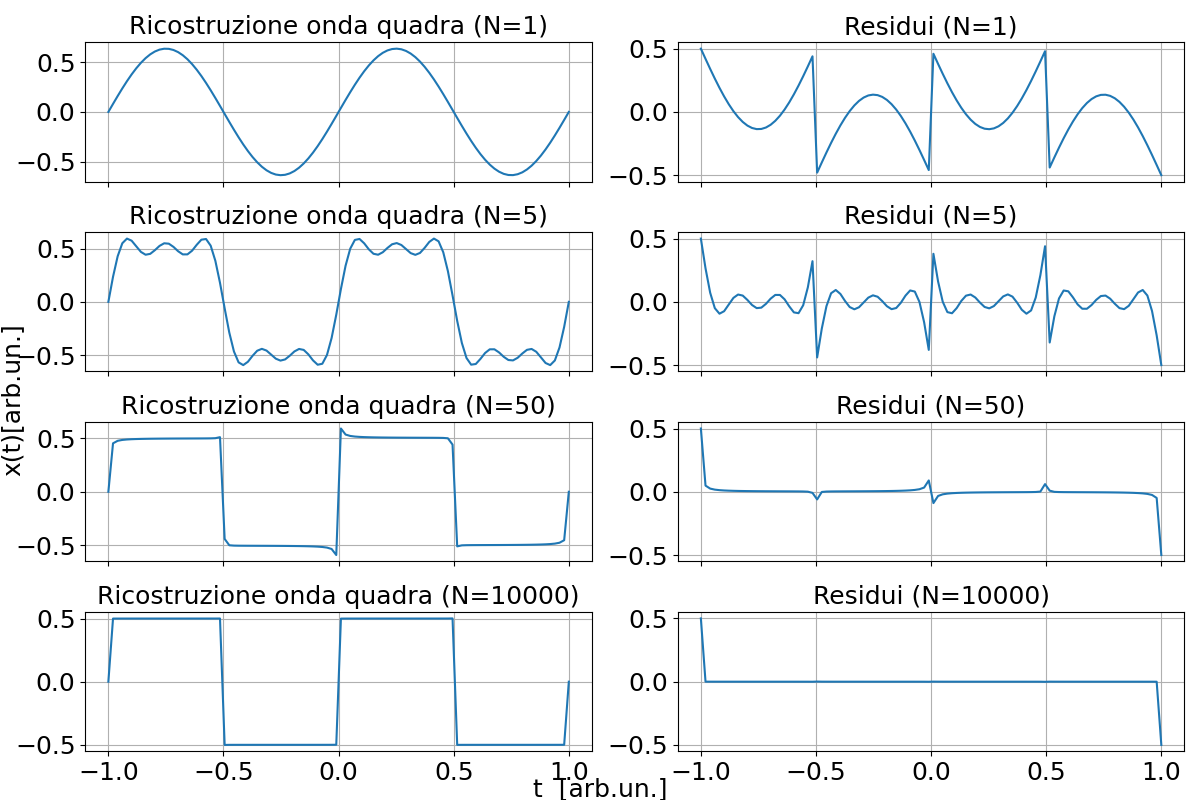
\includegraphics[width=0.85\textwidth]{fousquarewave1e2.png} % Replace with your image name
            \caption{A sinistra ricostruzione numerica dell'onda quadra Eq.($\ref{eq:quadra}$) su
                    due periodi con cento punti.
                    A destra residui tra onda analitica e la ricostruzione.
                    N è il numero a cui è stata troncata la serie.}
            \label{fig:quadra1e2}
        \end{figure}

        \noindent In Fig($\ref{fig:quadra1e2}$) e Fig($\ref{fig:quadra1e5}$) sono mostrate due ricostruzioni
        numeriche dell'onda quadra.
        All'aumentare dei termini $N$ della serie diminuisce la distranza tra onda analitica e serie 
        di seni.

        \noindent Si osserva che nel caso di Fig($\ref{fig:quadra1e2}$),
        la quale ha una risoluzione  peggiore, la deformazione dell'onda quadra assomiglia a quanto visto nelle esperienze 
        pratiche di laboratorio con l'oscilloscopio quando si usa il generatore di funzioni a
        frequenze sufficientemente alte.\\

        \begin{figure}[htbp]
            \centering
            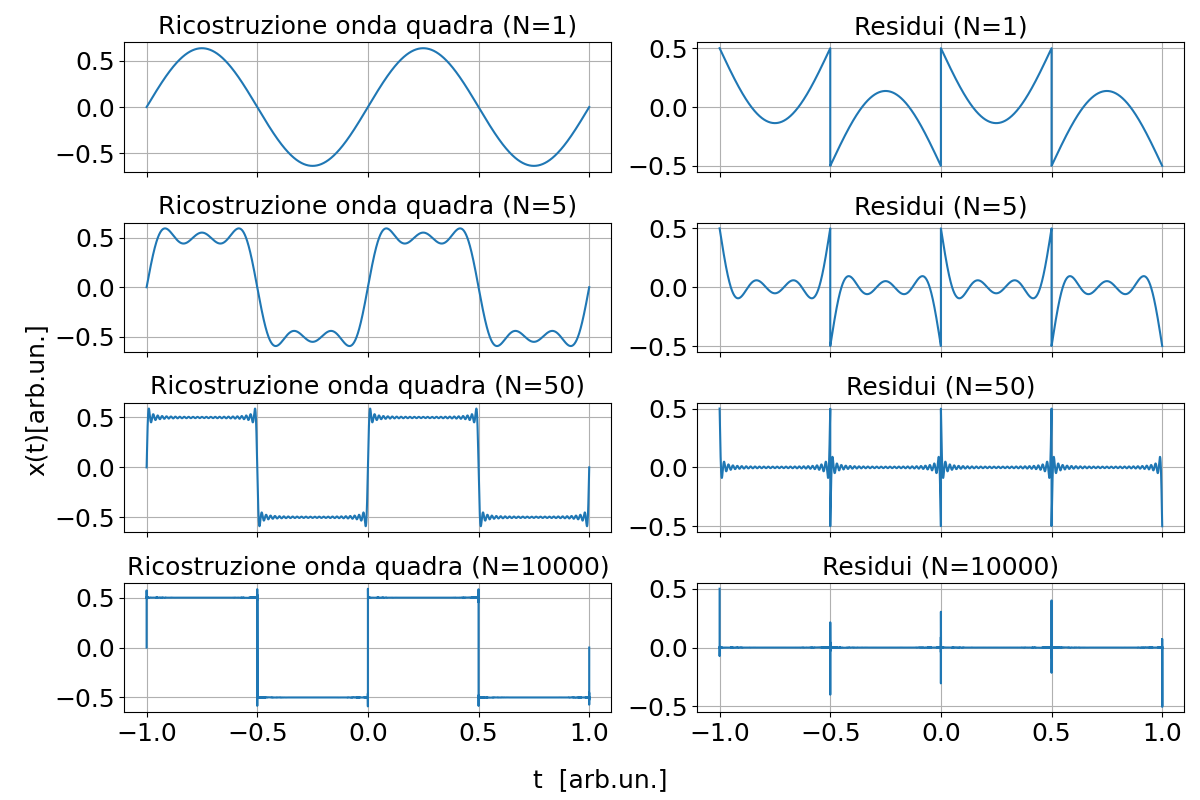
\includegraphics[width=0.85\textwidth]{fousquarewave1e5.png} % Replace with your image name
            \caption{A sinistra ricostruzione numerica dell'onda quadra Eq.($\ref{eq:quadra}$) su
                    due periodi con centomila punti.
                    A destra residui tra onda analitica e la ricostruzione.
                    N è il numero a cui è stata troncata la serie.}            \label{fig:quadra1e5}
        \end{figure}  
        
        
        \noindent La presenza di lati obliqui nei transienti è conseguenza di un sottocampionamento
        della ricostruzione, questo comporta che non c'è miglioramento dell'approssimazione all'aumentare dei termini 
        della serie.

        \noindent I residui nei punti iniziali e sui transienti non si annullano mai:  
        infatti non c'è convergenza semplice nei punti di discontinuità 
        della funzione, e quindi in corrispondenza di ognuno di
        questi  si trovano dei picchi. \newline \newline


    \subsection{Forme d'onda triangolari}
        \label{sez:trian}
        Un'onda triangolare alternata pari con ampiezza picco-picco unitaria
        e fase nulla è descitta dall' Eq.($\ref{eq:triangolare}$).
        \begin{equation}
            x(t) = \sum_{k=1,3,5...}^{\infty} \left(\frac{2}{k\pi}\right)^{2}\cos\left(k\omega t\right)
            \label{eq:triangolare}
        \end{equation}


        \begin{figure}[H]
            \centering
            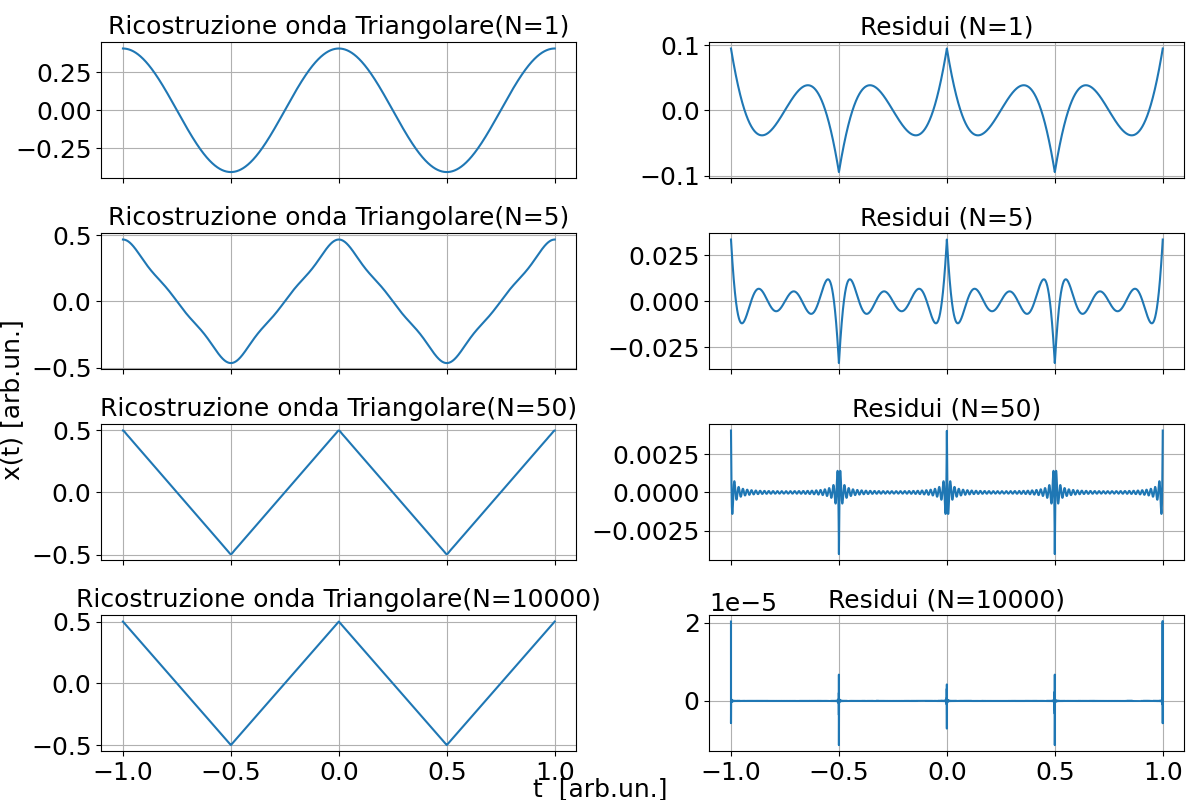
\includegraphics[width=0.85\textwidth]{foutriawave1e5.png} % Replace with your image name
            \caption{A sinistra ricostruzione numerica dell'onda triangolare
             Eq.($\ref{eq:triangolare}$) su due periodi con centomila punti.
            A destra residui tra onda analitica e la ricostruzione.
            N è il numero a cui è stata troncata la serie. }
            \label{fig:trian1e5}
        \end{figure}
        \noindent Differentemente da quanto accade per l'onda quadra, 
        in questo caso, nei punti in cui la derivata è discontinua 
        e nei punti al bordo c'è convergenza semplice anche se più lenta 
        che altrove.
        A tal proposito, si vedano grafici dei residui in Fig.($\ref{fig:trian1e5}$) e 
        Fig.($\ref{fig:trian1e2}$).
        Anche solo qualitativamente si osserva a entrambe le risoluzioni che 
        la convergenza all'onda analitica è più rapida dell'onda quadra,
         una migliore discussione di ciò avverrà in
        Sez.($\ref{sez:residui}$).
        \begin{figure}[H]
            \centering
            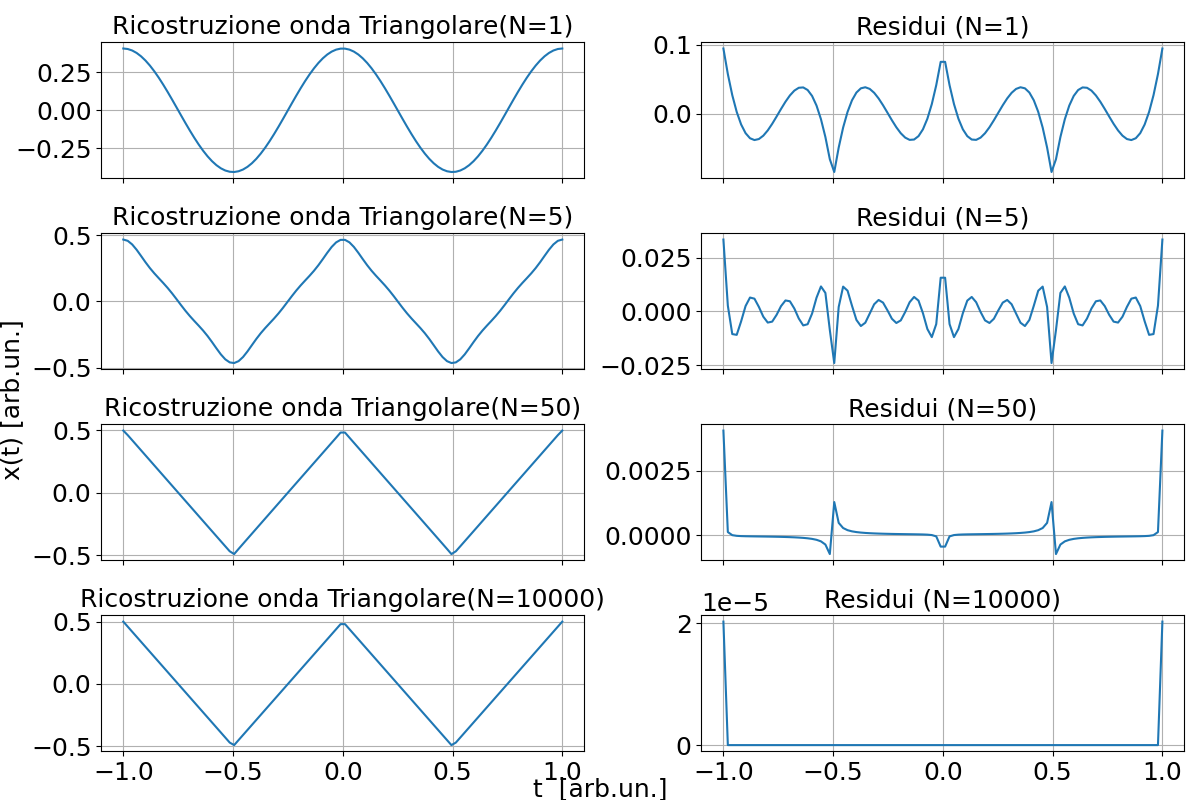
\includegraphics[width=0.85\textwidth]{foutriawave1e2.png} % Replace with your image name
            \caption{A sinistra ricostruzione numerica dell'onda triangolare
            Eq.($\ref{eq:triangolare}$)su due periodi con cento punti.
           A destra residui tra onda analitica e la ricostruzione.
           N è il numero a cui è stata troncata la serie. }
            \label{fig:trian1e2}
        \end{figure}        
        
        \noindent Per quanto riguarda l'utilizzo di diverse risoluzioni nei grafici, l'impiego di una risoluzione 
        minore comporta problemi nella convergenza solo nei punti iniziali
         e non nei punti di transiente; al contrario, l'impiego di una risoluzione 
        maggiore fa osservare dei picchi nei residui in prossimità dei transienti;
        questo è legato al particolare campionamento effettuato: 
        non mettere i punti di picco tra quelli che vengono campionati 
        comporta una deformazione della forma d'onda graficata che non viene osservata 
        nei residui.




    \subsection{Verifica di convergenza della serie}
    \label{sez:residui}
       
        La serie di Fourier delle rispettive onde dovrebbe convergere integralmente alle funzioni analitiche.
        La velocità di convergenza rispetto al numero 
        di iterazioni è diversa per le forme d'onda come si può vedere 
        in Fig.($\ref{fig:res1}$).\\ 
        Quando il campionamento avviene su numero sufficientemente
        piccolo di periodi,nel caso in questione 50 campionamenti al periodo,
          non c'è più convergenza integrale tra la funzione semplice, definita sugli 
        intervalli dalla serie di Fourier, e la funzione analitica:con ogni
        probabilità questo è dovuto al transiente che non è adeguatamente approssimato.
        Inaspettatamente ,si osserva che entrambe le onde compiono delle "oscillazioni smorzate":
        la convergenza dovrebbe migliorare all'aumentare dei termini delle serie,
        ma localmente questo non è verificato, si veda Fig.($\ref{fig:res2}$).
        

        \begin{figure}[H]
            \centering
            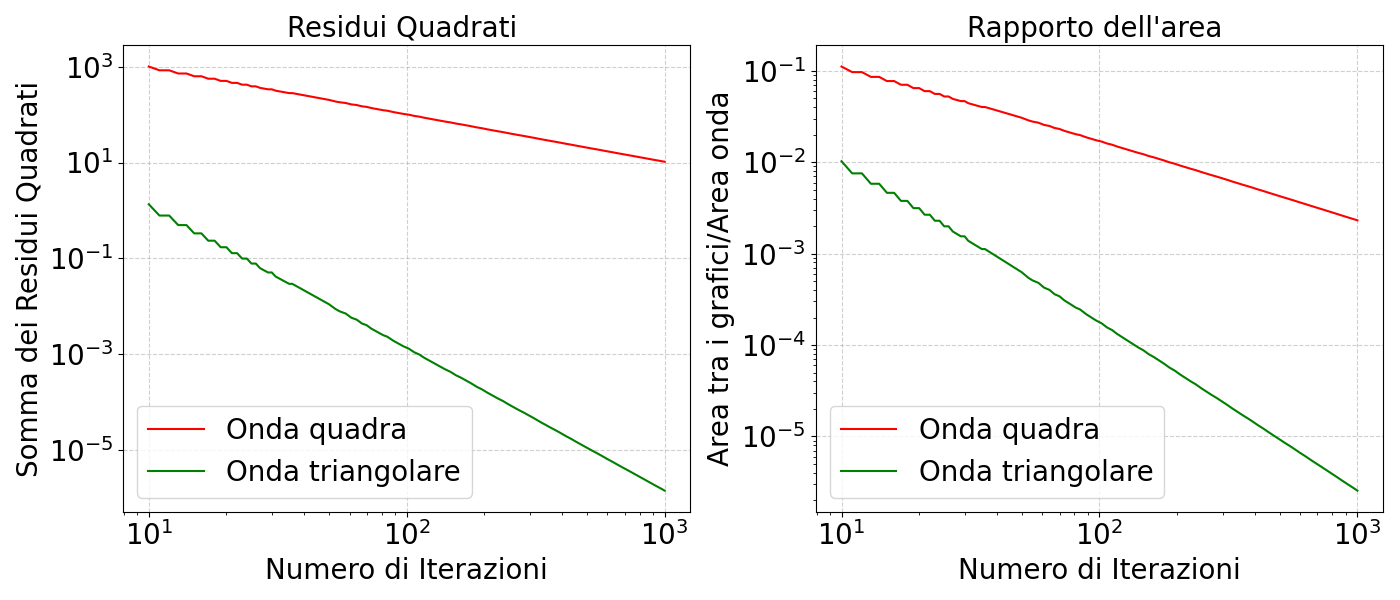
\includegraphics[width=0.85\textwidth]{residuals1.png} % Replace with your image name
            \caption{Nella figura simulazione numerica sono stati usati cento milioni di campionamenti presi tra due periodi.}
            \label{fig:res1}
        \end{figure}

      

        \begin{figure}[H]
            \centering
            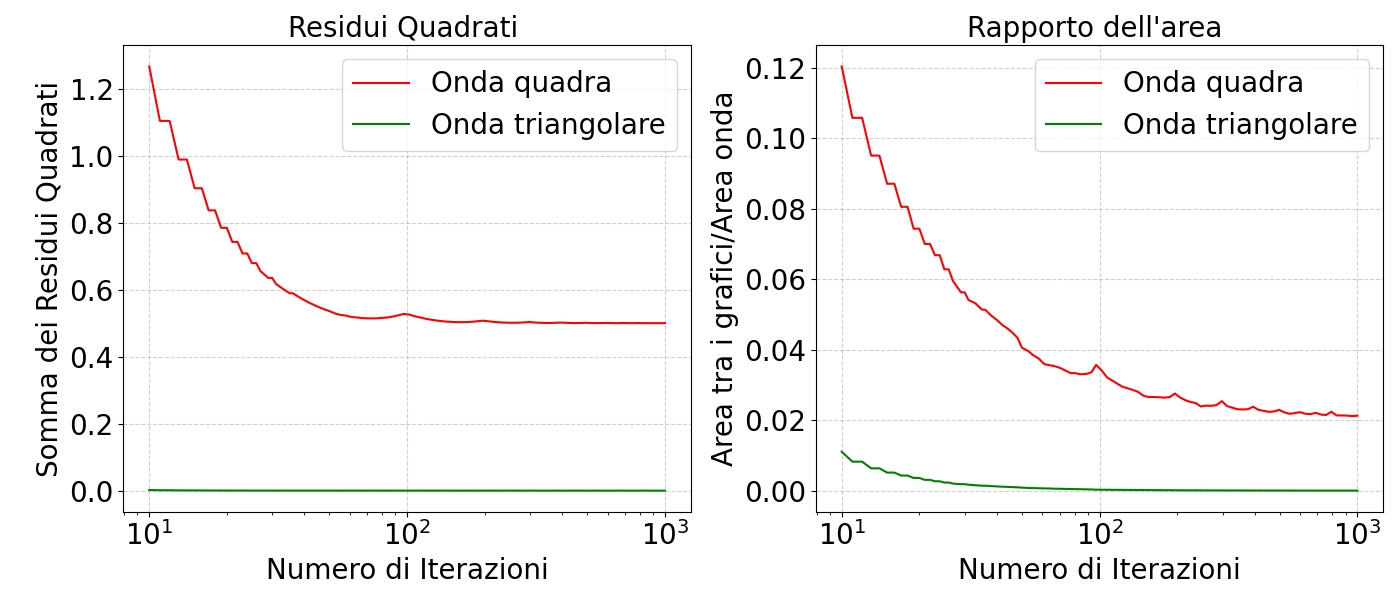
\includegraphics[width=0.85\textwidth]{residuals2.png} % Replace with your image name
            \caption{Nella figura simulazione numerica sono stati usati 100 campionamenti presi tra due periodi.}
            \label{fig:res2}
        \end{figure}

    \subsection{Treni di impulsi}
    Un treno di impulsi pari con ampiezza picco-picco unitaria e fase nulla è descitta
    dall' Eq.($\ref{eq:ciufciuf}$).

    \begin{equation}
        x(t) = \sum_{k=1,3,5...}^{\infty} \left(\frac{2}{k\pi}\right)\sin\left(k\pi\delta\right)\cos\left(k\omega t\right)
        \label{eq:ciufciuf}
    \end{equation}
    $\delta$ è il rapporto tra massimo e minimo dell'onda.
    Come si può vedere in Fig.($\ref{fig:ciufciuf1} $) e in Fig.($\ref{fig:ciufciuf2} $),
    è possibile fare le stesse identiche osservazioni fatte in Sez(\ref{sez:quadra}).
    \begin{figure}[H]
        \centering
        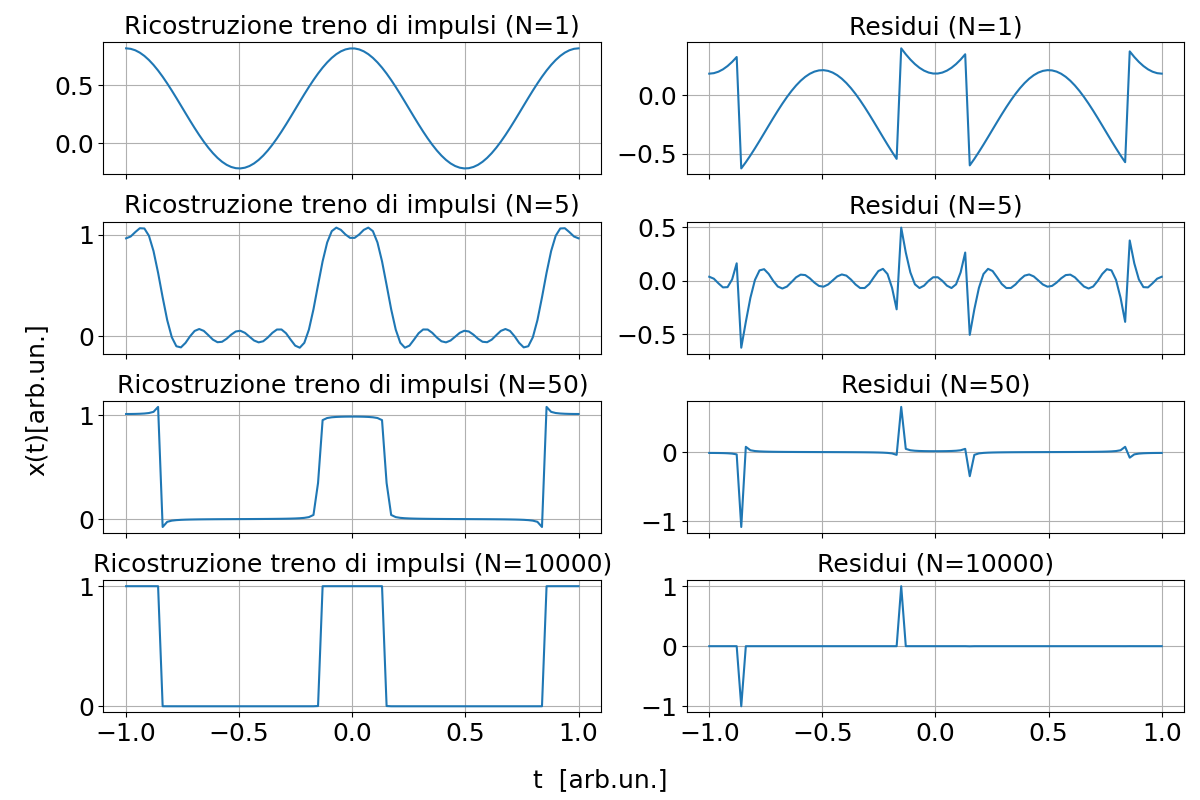
\includegraphics[width=0.85\textwidth]{foupulsetrainwave1e2.png} % Replace with your image name
        \caption{A sinistra ricostruzione numerica del treno di impulsi
        Eq.($\ref{eq:ciufciuf}$)su due periodi con cento punti.
        A destra residui tra onda analitica e la ricostruzione.
        N è il numero a cui è stata troncata la serie. }
        \label{fig:ciufciuf1}
    \end{figure}

    \begin{figure}[H]
        \centering
        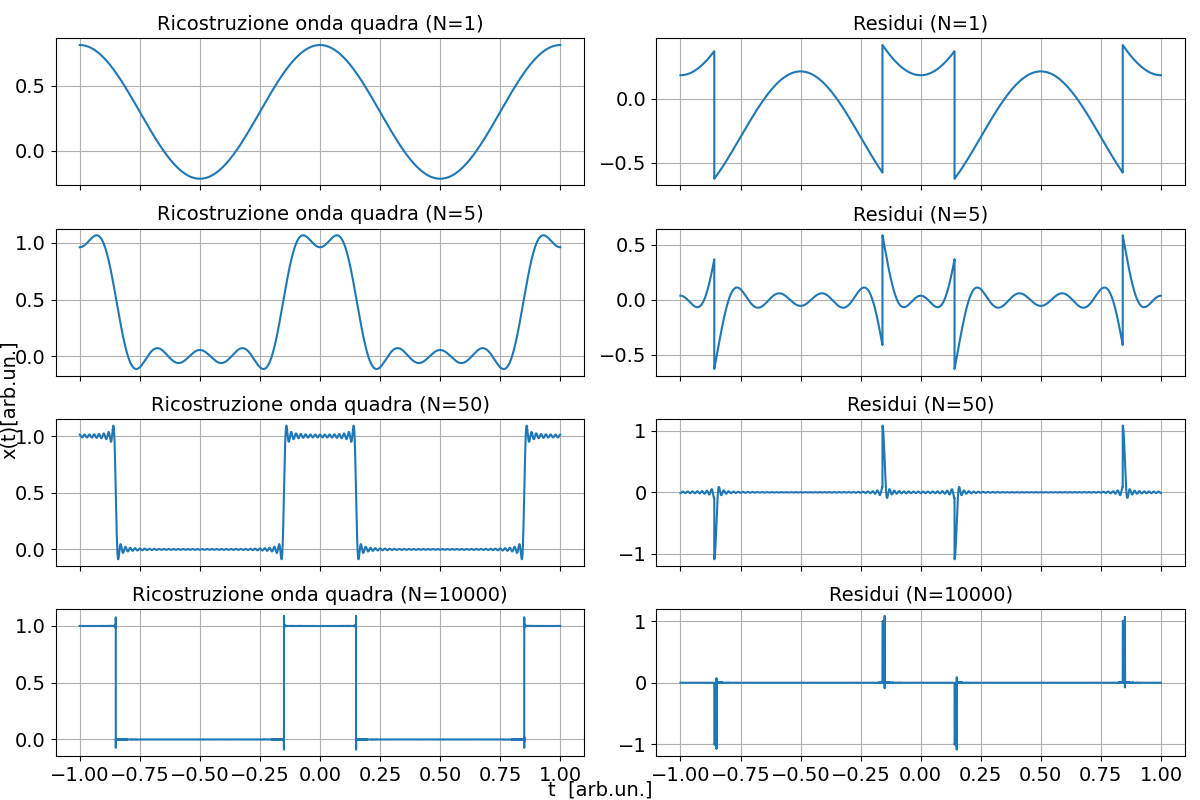
\includegraphics[width=0.85\textwidth]{foupulsetrainwave1e5.png} % Replace with your image name
        \caption{A sinistra ricostruzione numerica del treno di impulsi
        Eq.($\ref{eq:ciufciuf}$)su due periodi con centomila punti.
        A destra residui tra onda analitica e la ricostruzione.
        N è il numero a cui è stata troncata la serie. }
        \label{fig:ciufciuf2}
    \end{figure}



\section{Filtro passa basso e filtro passa alto}
    \label{sez:filt}
    Un filtro passa basso di frequenza di taglio $f_T$, che riceve un segnale sinusoidale, di 
    frequenza angolare $\omega$,lo riscala di un fattore $G$ e lo sfasa di un 
    angolo $\phi$ come dato da Eq.($\ref{eq:lpf}$).
        \begin{equation}
            f = \frac{\omega}{2\pi}, \quad 
            G(f) = \frac{1}{\sqrt{1 + \left(\frac{f}{f_T}\right)^2}}, \quad 
            \phi = \arctan\left(\frac{-f}{f_T}\right)
            \label{eq:lpf}
        \end{equation}
    Un filtro passa alto di frequenza di taglio $f_T$, che riceve un segnale sinusoidale, di 
    frequenza angolare $\omega$,lo riscala di un fattore $G$ e lo sfasa di un 
    angolo $\phi$ come dato da Eq.($\ref{eq:hpf}$).
        \begin{equation}
            f = \frac{\omega}{2\pi}, \quad 
            G(f) = \frac{1}{\sqrt{1 + \left(\frac{f_T}{f}\right)^2}}, \quad 
            \phi(f)= \arctan\left(\frac{f_T}{f}\right)
            \label{eq:hpf}
        \end{equation}

    Dunque le equazioni per le onde passanti per ciascuno dei filtri si trovano
    moltiplicando ciascun termine della sommatoria per il rispettivo 
    $G \left( k\omega,f_T\right)$ e sommando il termine $\phi \left( k\omega,f_T\right)$ 
    all'interno della sinusoide o cosinusoide. $G$ e $\phi$ hanno significato di Eq.($\ref{eq:lpf}$)
    o Eq($\ref{eq:hpf}$) dipendentemente dal filtro del contesto.

    Tutte le simulazioni di questa sezione sono state fatte assegnando alle onde periodo unitario.
      
    
    \subsection{Onda quadra}
    Le funzioni descriventi il segnale in uscita o in ingresso da un filtro passa basso
    o passa alto, i quali in ingresso hanno un'onda quadra, 
    sono date dal procedimento descritto i Sez.($\ref{sez:filt}$).
        \subsubsection{Filtro passa basso}
            \label{sez:int_quadra}

            E' possibile fare le stesse considerazioni riguardanti 
            il numero di termini della serie impiegati, i transienti e il campionamento come
            in Sez.($\ref{sez:trian}$), in quanto la curva che viene apprissimata è 
            continua (vedi Fig($\ref{fig:shark1e2}$) e Fig($\ref{fig:shark1e5}$)).
                    \begin{figure}[H]
                        \centering
                        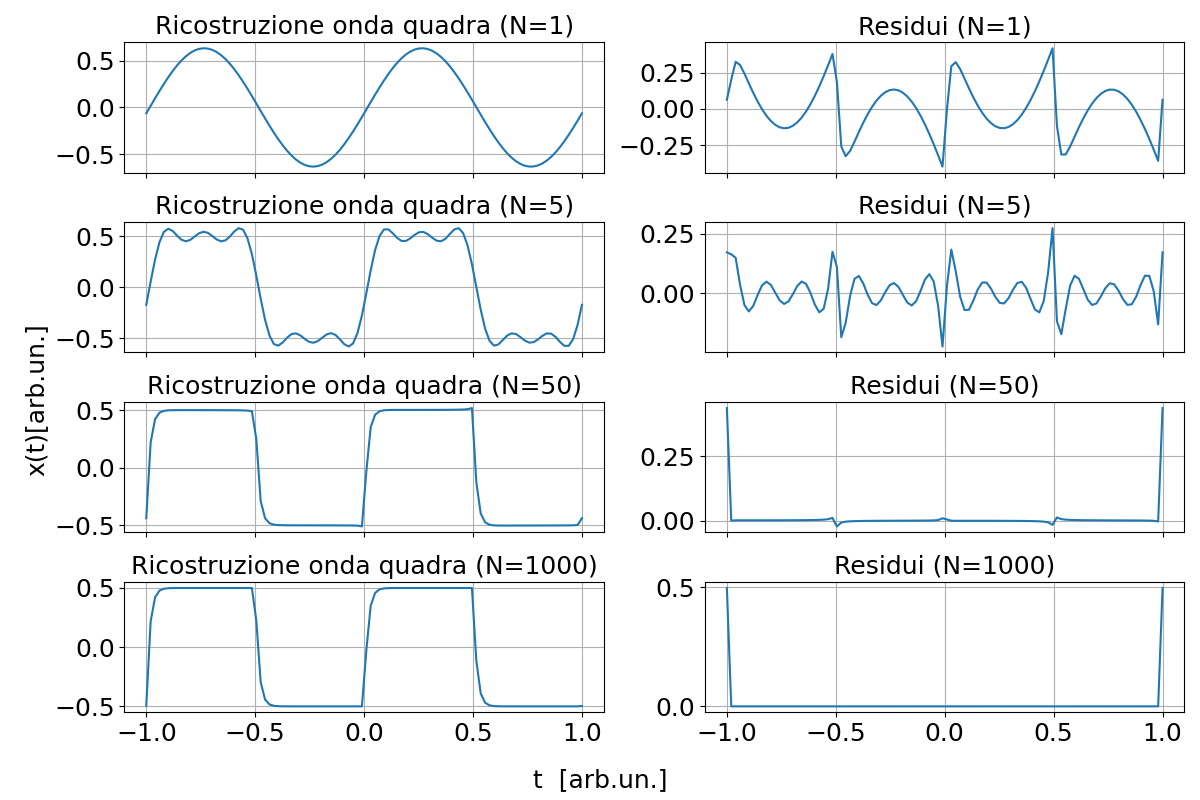
\includegraphics[width=0.85\textwidth]{fousharkfins1e2.png} % Replace with your image name
                        \caption{A sinistra c'è l'onda a pinna di squalo.
                        A destra c'è il grafico dei residui.
                        La risoluzione utilizzata è stata di cento punti su due periodi.}
                        \label{fig:shark1e2}
                    \end{figure}
                    \begin{figure}[H]
                        \centering
                        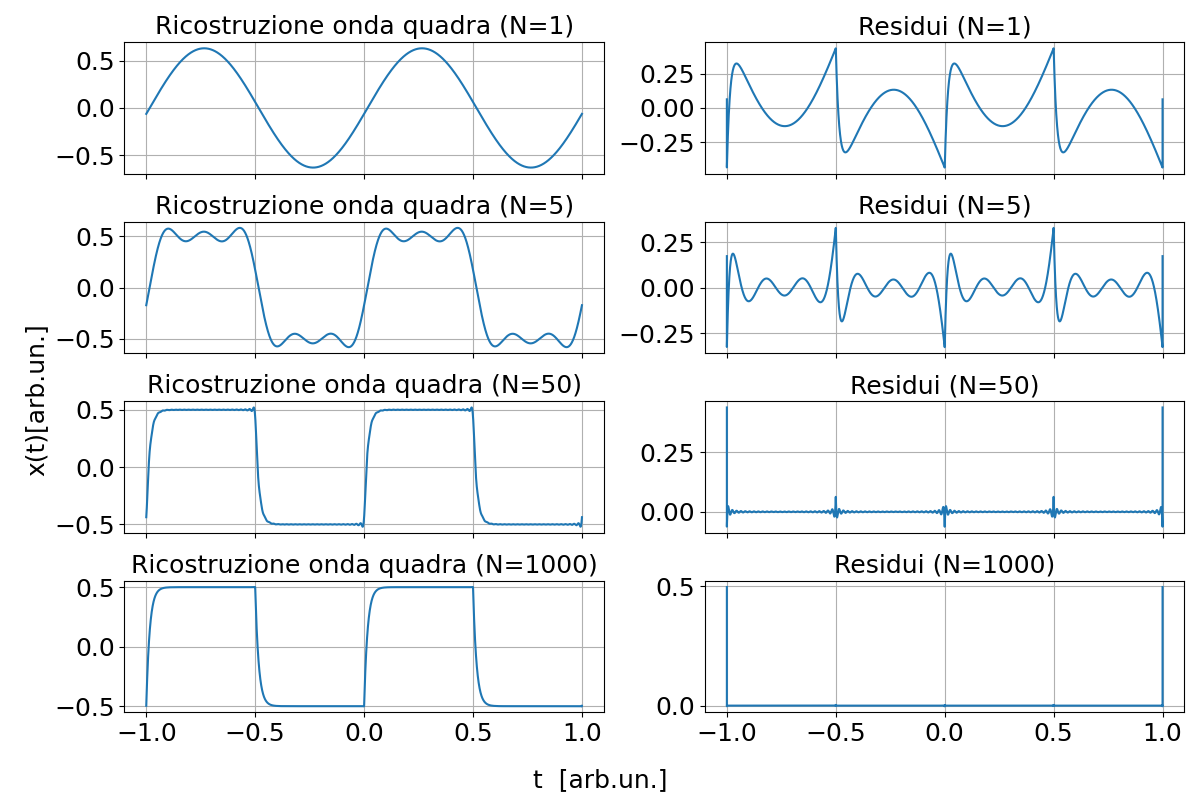
\includegraphics[width=0.85\textwidth]{fousharkfins1e5.png} % Replace with your image name
                        \caption{A sinistra c'è l'onda a pinna di squalo.
                        A destra c'è il grafico dei residui.
                        La risoluzione utilizzata è stata di centomila punti su due periodi.
                        La serie di Fourier è stata troncata al termine $N=10000$.}
                        \label{fig:shark1e5}
                    \end{figure}
                Si può simulare il comportamento di  un filtro al
                variare della frequenza in ingresso: per semplicità 
                la simulazione è stata fatta tenendo fissa la frequenza dell'onda e 
                variando la frequenza di taglio, si veda Fig.($\ref{fig:sharkft}$).
                    \begin{figure}[H]
                        \centering
                        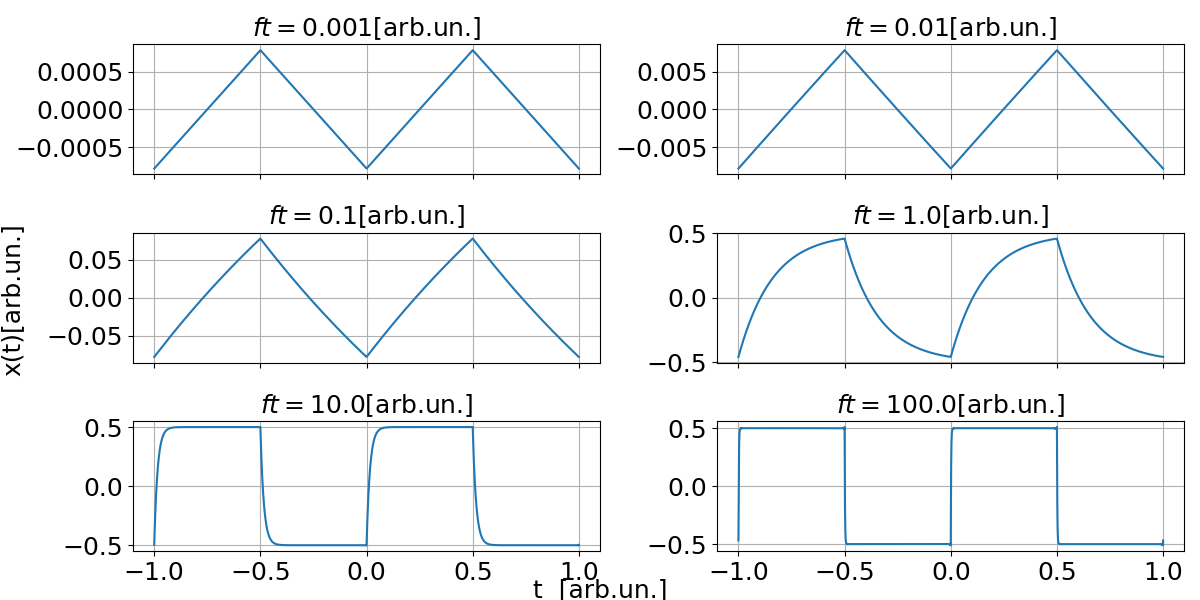
\includegraphics[width=0.85\textwidth]{fousharkfinsfts1.png} % Replace with your image name
                        \caption{Onde a pinna di squalo al variare della frequenza di taglio.
                        La risoluzione utilizzata è stata di centomila punti su due periodi.
                        La serie di Fourier è stata troncata al termine $N=10000$.}
                        \label{fig:sharkft}
                    \end{figure}

                \noindent Quanto simulato e mostrato in Fig.($\ref{fig:sharkft}$)
                è in accordo con quanto visto in laboratorio: 
                al decrescere della frequenza di taglio rispetto alla frequenza dell'onda quadra
                l'onda tende a diventare triangolare e la sua ampiezza diminuisce; viceversa,
                l'onda tenda a divenire quadra, ossia il segnale in ingresso tende a 
                rimanere inalterato.
            
            
            \subsubsection{Filtro passa alto}
                In Fig($\ref{fig:der_square}$) si simula il passaggio di un'onda quadra
                attraverso un filtro passa alto: si  può osservare specialmente 
                nel caso $ft=0.1$[arb.un.] la stessa forma d'onda osservata collegando 
                l'oscilloscopio in modalità AC al generatore di funzioni.
                    \begin{figure}[H]
                        \centering
                        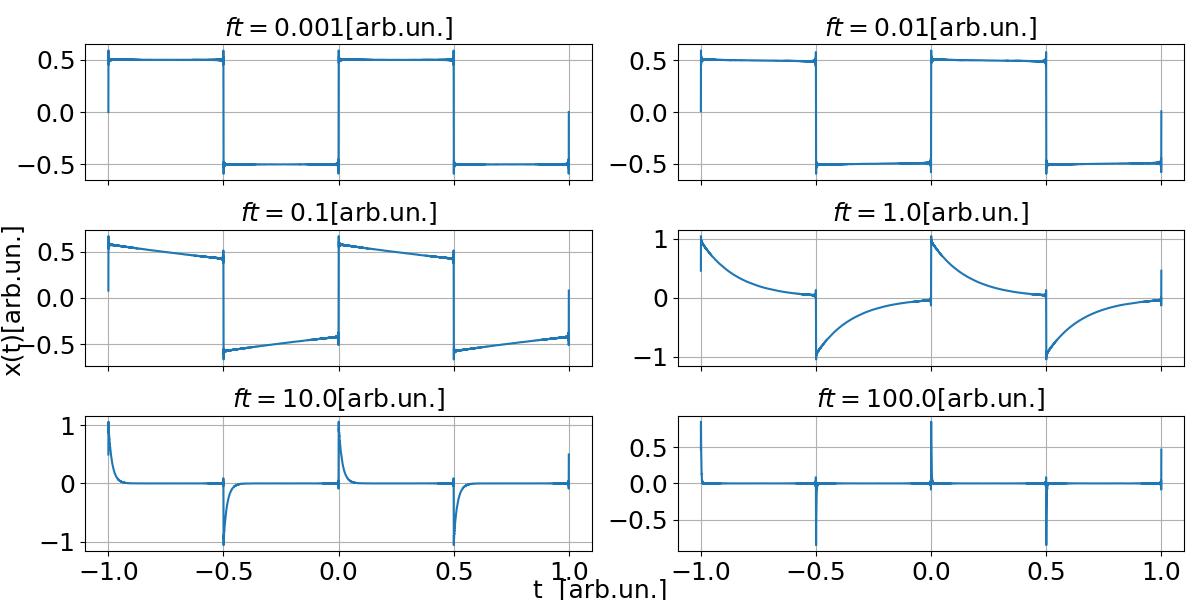
\includegraphics[width=0.85\textwidth]{der_square.png} % Replace with your image name
                        \caption{Simulazione di filtro passa alto con onda quadra.
                        La risoluzione utilizzata è stata di centomila punti su due periodi.
                        La serie di Fourier è stata troncata al termine $N=10000$.}
                        \label{fig:der_square}
                    \end{figure}


    \subsection{Onda triangolare}
    Le funzioni descriventi il segnale i uscita o in ingresso da un filtro passa basso
    o passa alto, i quali in ingresso hanno un'onda triangolare, 
    sono date dal procedimento descritto i Sez.($\ref{sez:filt}$).
        \subsubsection{Integratore}
            
            In Fig.($\ref{fig:trilpf}$) viene riportato il comportamento di un filtro passa
            basso per un' onda triangolare. Valgono tutti i commenti precedentemente in 
            Sez.($\ref{sez:int_quadra}$)
            \begin{figure}[H]
                \centering
                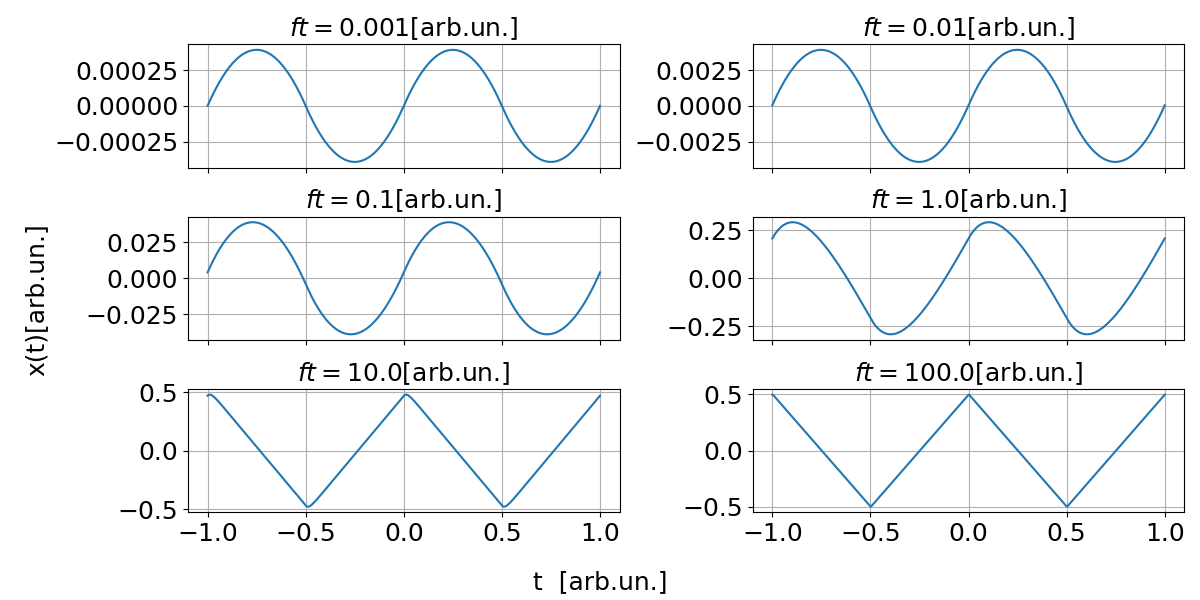
\includegraphics[width=0.85\textwidth]{integ_trian.png} % Replace with your image name
                \caption{Per la ricostruzione della forma d'onda è stato adottato 
                il procedimento descritto in Sez.($\ref{sez:filt}$).
                La risoluzione utilizzata è stata di centomila punti su due periodi.
                La serie di Fourier è stata troncata al termine $N=10000$.}
                \label{fig:trilpf}
            \end{figure}
        \subsubsection{Derivatore}
            In questo caso (vedi Fig.($\ref{fig:trihpf}$)), si osserva che la forma d'onda 
            triangolare passante per un filtro passa alto coincide con quella simulata 
            per un filtro passa basso attraversato da un'onda quadra(vedi Fig($\ref{fig:sharkft}$))
                \begin{figure}[H]
                    \centering
                    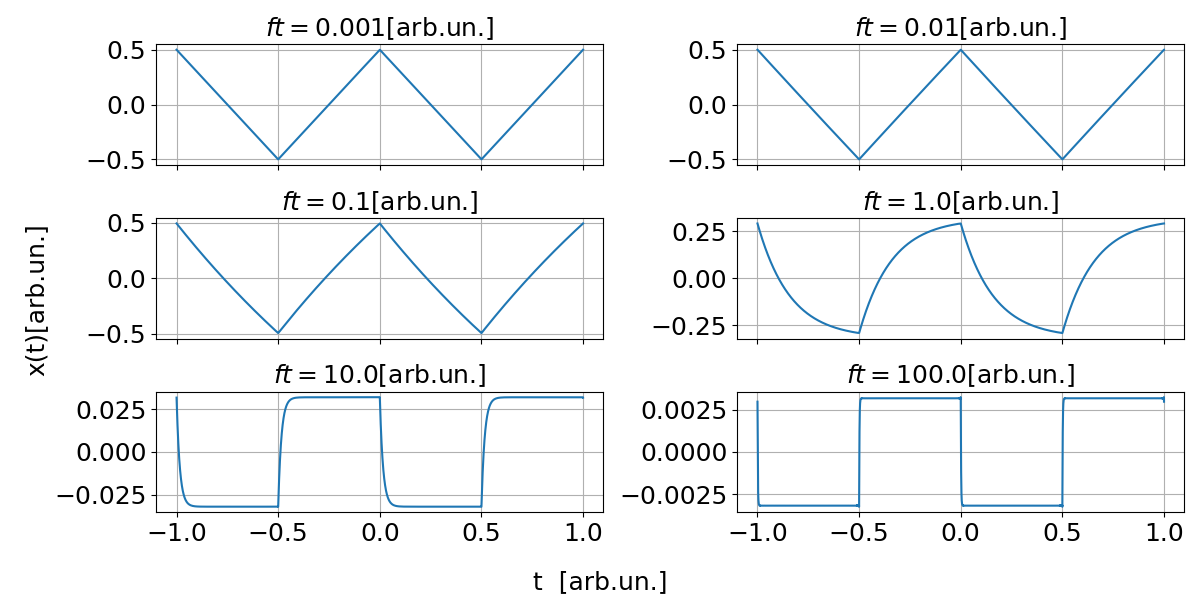
\includegraphics[width=0.85\textwidth]{der_trian.png} % Replace with your image name
                    \caption{Per la ricostruzione della forma d'onda è stato adottato 
                    il procedimento descritto in Sez.($\ref{sez:filt}$).
                    La risoluzione utilizzata è stata di centomila punti su due periodi.
                    La serie di Fourier è stata troncata al termine $N=10000$.}
                    \label{fig:trihpf}
                \end{figure}


    \subsection{Treno di impulsi}
    Le funzioni descriventi il segnale i uscita o in ingresso da un filtro passa basso
    o passa alto, i quali in ingresso hanno un treno di impulsi, 
    sono date dal procedimento descritto i Sez.($\ref{sez:filt}$).
  
            \subsubsection{Integratore}
            Le osservazioni che si possono fare in questo caso sono già state fatte 
            nella trattazione dell'onda quadra Sez.($\ref{sez:int_quadra}$).
            In Fig.($\ref{fig:int_train}$) viene riportato il segnale integrato di un treno di impulsi.
                Per facilità di rappresentazione e facilitare possibili manipolazioni
                nello studio della forma, è stato scelto di tenere compresa la forma 
                d'onda in un intervallo unitario centrato in zero.
                Se questo non fosse stato fatto appositamente, la forma d'onda, non 
                essendo alternata, non avrebbe spontaneamente, eccetto che nel caso 
                in cui si fosse ricondotti a un'onda quadra, rispettato questa richiesta.
        
                    \begin{figure}[H]
                        \centering
                        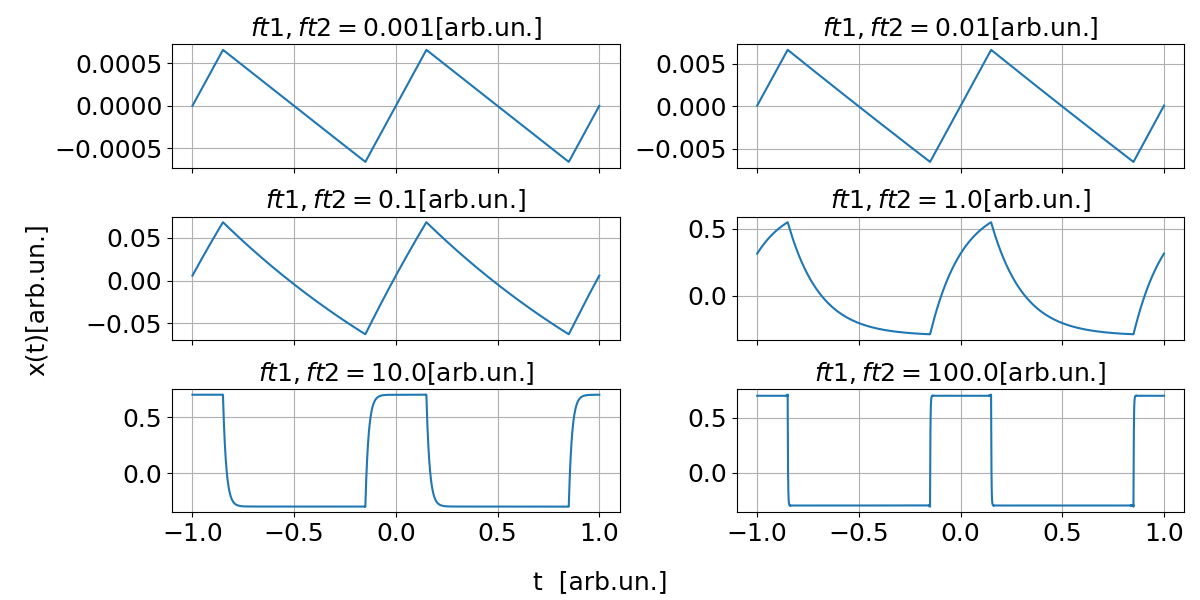
\includegraphics[width=0.85\textwidth]{int_train1.png} % Replace with your image name
                        \caption{Per la ricostruzione della forma d'onda è stato adottato 
                        il procedimento descritto in Sez.($\ref{sez:filt}$).
                        La risoluzione utilizzata è stata di centomila punti su due periodi.
                        E' stato fatto un troncamento al tremine 10000
                        nello sviluppo della serie di seni.}
                        \label{fig:int_train}
                    \end{figure}               

            \subsubsection{Derivatore}
                In Fig.($\ref{fig:der_train}$) viene riportato il segnale derivato di un treno di impulsi.     
                    
                    \begin{figure}[H]
                        \centering
                        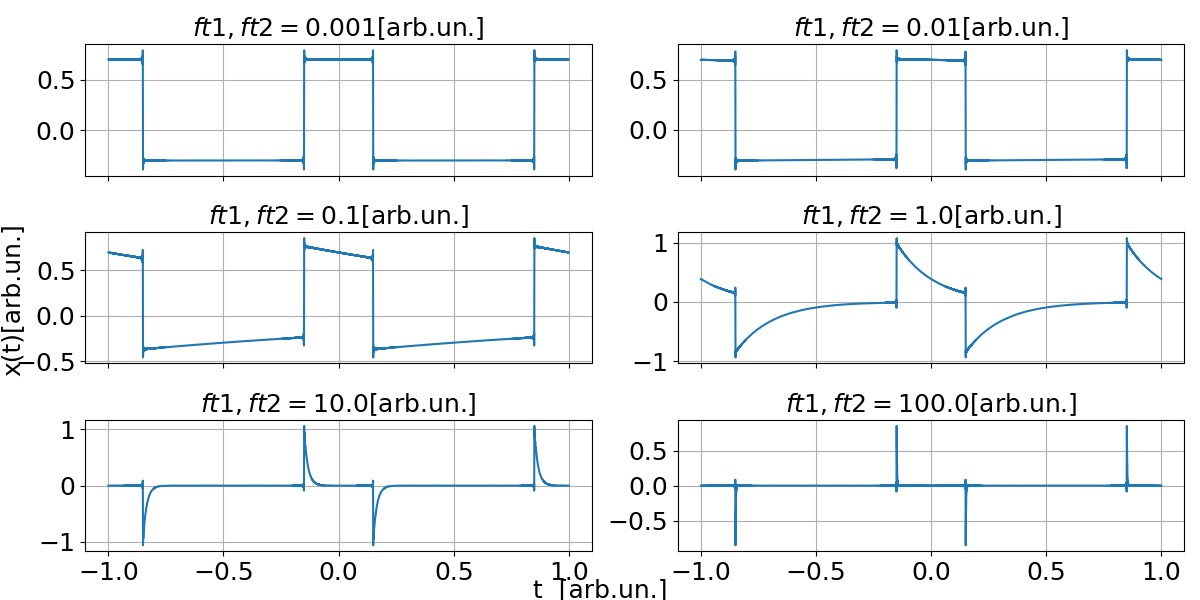
\includegraphics[width=0.85\textwidth]{der_train.png} % Replace with your image name
                        \caption{Per la ricostruzione della forma d'onda è stato adottato 
                        il procedimento descritto in Sez.($\ref{sez:filt}$).
                        La risoluzione utilizzata è stata di centomila punti su due periodi.
                        Sono stati usati 10000 termini della serie di seni.}
                        \label{fig:der_train}
                    \end{figure}    

            \subsubsection{Filtro passa banda}
                In Fig.($\ref{fig:band_train}$) si simula il comportamento di un treno di impulsi
                attraversante un filtro passa banda.
                \begin{figure}[H]
                    \centering
                    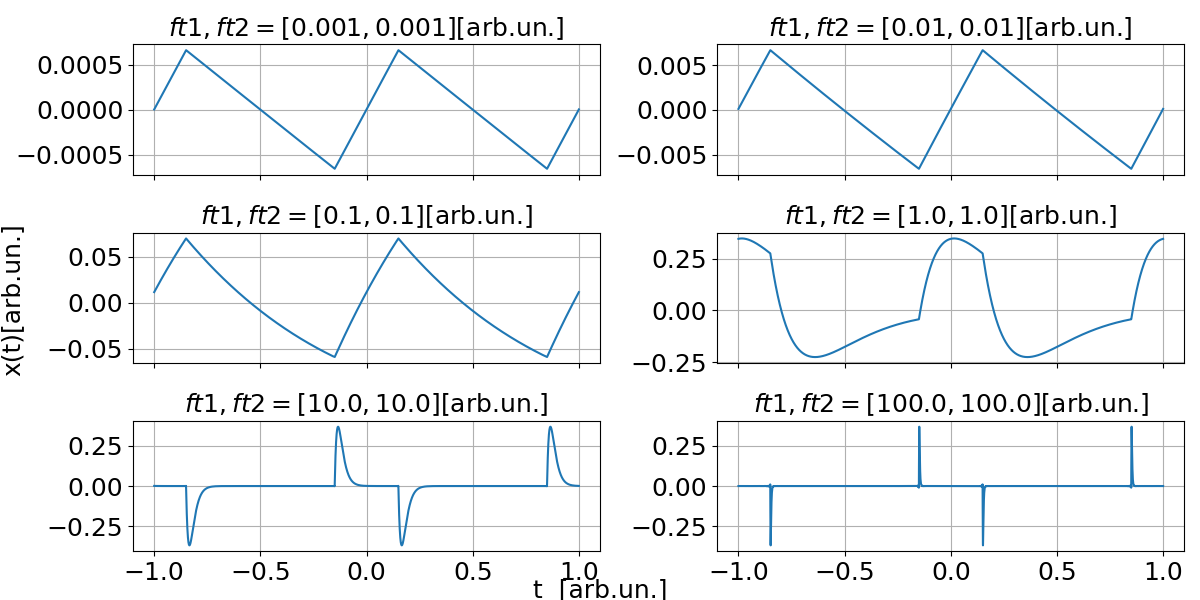
\includegraphics[width=0.85\textwidth]{band_train.png} % Replace with your image name
                    \caption{Per la ricostruzione della forma d'onda è stato adottato 
                    il procedimento descritto in Sez.($\ref{sez:filt}$).
                    La risoluzione utilizzata è stata di centomila punti su due periodi.
                    Sono stati usati 10000 termini della serie di seni.}
                    \label{fig:band_train}
                \end{figure}


\section{Best fit dei dati acquisiti con Arduino}
    Sono stati realizzati dei best fit con le funzioni ricostruite
    dei i dati di un filtro passa-basso che acquisiti
    in laboratorio con Arduino. 
    Il filtro passa-basso, con i valori nominali della resistenza $R$ e della capacità $C$ del
    condensatore riportati in Tab.(\ref{tab:val_nom}),
    \begin{table}[htbp]
        \centering
        \begin{tabular}{c c}
            \hline
            $R$ [k$\Omega$] & $C$ [$\mu$F] \\
            \hline
            $0.68 \pm 0.03$ & $1.0 \pm 0.2$ \\
            \hline
        \end{tabular}
        \caption{Tabella dei valori nominali della resistenza e della capacità del condensatore con cui abbiamo realizzato il filtro passa-basso in laboratorio.}
        \label{tab:val_nom}
    \end{table}
    doveva essere caratterizzato da una frequenza di taglio che è
     data dalla formula $f_T = \frac{1}{2 \pi RC}$, che nel nostro caso vale:
    $$
    f_T = (0.23 \pm 0.06) \text{ mHz}.
    $$
    Per tutti i best-fit realizzati abbiamo troncato la serie di Fourier al termine $N=1000$. Questo è stato necessario per far eseguire il 
    best-fit in tempi ragionevoli.
    Come incertezza sulle misure di potenziale è stata
    presa la deviazione standard campione di un set di dati, raccolti con Arduino, delle misure
    della differenze di potenziale tenuta costante \cite{Antonacci_Sermi2024}.
    Per la natura statistica dell'incertezza è stato dunque assunto \emph{absolute\_ sigma=True},
    eccetto dove specificato il contrario.
    \subsection{Onda quadra}
            E' stato realizzato il best-fit dei minimi quadrati
            di un set di dati compatibile con un'onda quadra.
            Il modello con cui fare il best-fit è descritto dall'Eq.($\ref{eq:fit_square}$).
                \begin{equation}
                    V(t) = \left[a\sum_{k=1,3,5...}^{1000} \frac{2}{k\pi}\sin\left(k\omega (t+\delta)\right)\right] +c
                    \label{eq:fit_square}
                \end{equation}
            Si osserva che trascurare o meno i punti sui transienti è incisivo
            sul risultato di best-fit come si può vedere in Fig.($\ref{fig:bestfit_square}$).
            Quello che accade è che considerando i transienti non sarebbe legittimo
            applicare l'argoritmo di best-fit Levenberg-Marquardt in quanto l'errore 
            sulla variabile indipendente non è trascurabile: implementare la  tecnica 
            dell'errore efficare, a causa della divergenza della derivata della funzione, equivale
            a trascurare le misure sui transienti.
            E' stato dunque ragionevole utilizzare \emph{absolute\_ sigma=True}
            nel primo best fit, e \emph{absolute\_ sigma=False} nel secondo.
            Dal $\chi^2$ risulta che l'errore è stato sovrastimato. 
            I parametri ottenuti sono riportati in Tab.(\ref{tab:bestfit_square}).
            In Fig.($\ref{fig:bestfit_square}$) sono riportati i dati con il best fit e 
            i residui.
            

            \begin{figure}[H]
                \centering
                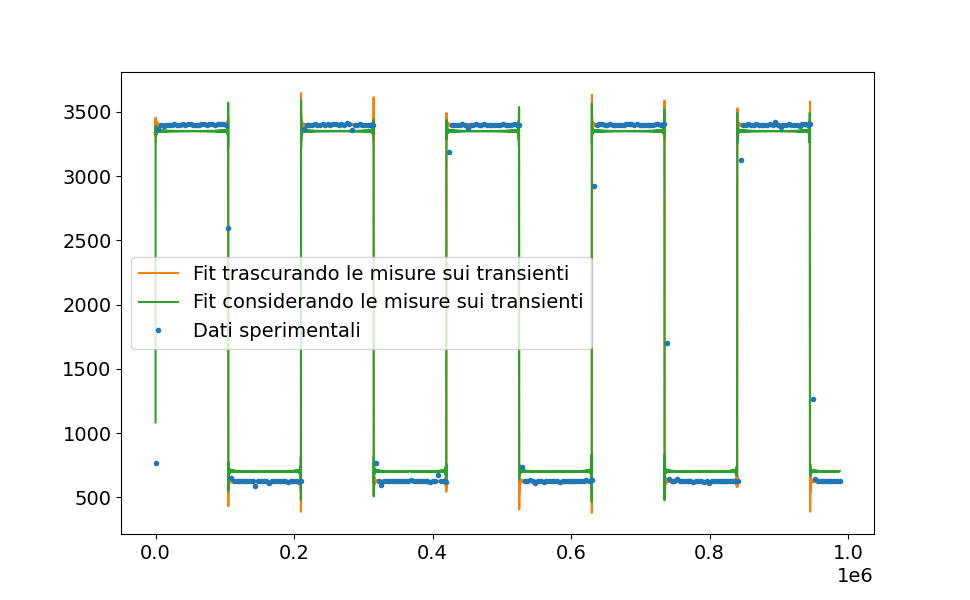
\includegraphics[width=0.85\textwidth]{bestfit_squarewave.png} % Replace with your image name
                \caption{Bestfit di un'onda quadra campionata tramite la scheda Arduino.}
                \label{fig:bestfit_square}
            \end{figure}     
            

            \begin{table}[H]
                \centering
                \begin{tabular}{ccc}
                    \hline
                     & Fit trascurando i transienti & Fit considerando i transienti \\
                    \hline
                    $\omega$ [rad/s]        & $29.923 \pm 0.001$    & $29.930\pm 0.003$ \\
                    $\delta$ [$\mu$s]       & $-35\pm 24$           & $-42\pm 19$ \\
                    a [arb.un]              & $2774 \pm 1$          & $2647 \pm 47$ \\
                    c [arb.un]              & $2012.8 \pm 0.7$      & $2026 \pm 23$ \\
                    $\chi^{2}_{norm}$ & 0.01 & 14 \\
                    \hline
                \end{tabular}
                \caption{Parametri ottenuti nei best-fit dell'onda quadra eseguito utilizzando il modello descritto dall'eq.($\ref{eq:fit_square}$).}
                \label{tab:bestfit_square}
            \end{table}
            

            
    \subsection{Onda a pinna di squalo}
        E' stato realizzato il best-fit dei minimi quadrati
        di quattro set di dati compatibile con un'onda a pinna di squalo.
        Il modello con cui fare il best-fit è descritto dall'Eq.($\ref{eq:fit_shark}$).
                \begin{equation}
                    x(t) = \left[a\sum_{k=1,3,5...}^{1000} \frac{2G(f,f_T)}{k\pi}\sin\left(k\omega (t+\delta)+\phi(f,f_T)\right)\right] +c
                    \label{eq:fit_shark}
                \end{equation} 
        I parametri ottenuti sono riportati in Tab.(\ref{tab:bestfit_params}).%%%%%%%%%%%%%CHANGE TABLE 
        In Fig.($\ref{fig:bestfit_shark.fig}$) sono riportati i dati con il best fit e 
        i residui: si osserva che, fatta eccezione del primo grafico,la frequenza di taglio aspettata è compatibile entro una 
        barra di errore con quelle stimate. 

                \begin{figure}[H]
                    \centering
                    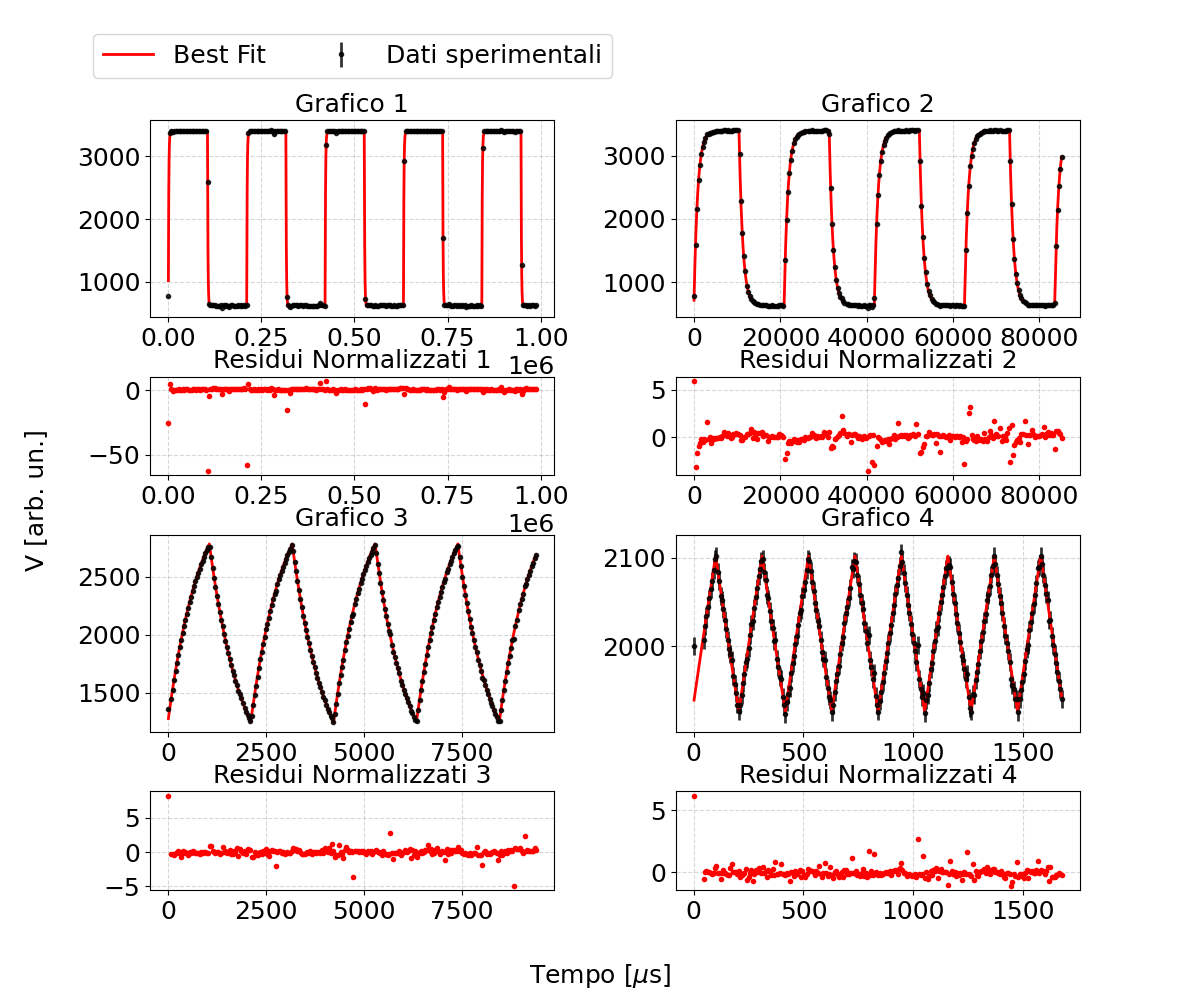
\includegraphics[width=0.85\textwidth]{bestfit_sharkfins.png} % Replace with your image name
                    \caption{Grafico di bestfit nel caso di un'onda a pinna di squalo
                    }
                    \label{fig:bestfit_shark.fig}
                \end{figure}     

                \begin{table}[H]
                    \centering
                    \begin{tabular}{cccccc}
                        \hline
                         & Grafico1 & Grafico2 & Grafico3 & Grafico4 \\
                        \hline
                        $\omega$ [rad/s]    & $0.29839 \pm 0.0005$      & $300.691\pm 0.009$    & $2970.0 \pm 0.4$      & $29669.8\pm 0.2$ \\
                        $f_T$ [mHz]         & $0.140 \pm 0.001$         & $0.1864 \pm 0.0004$   & $0.189 \pm 0.002$     & $0.1 \pm 0.1$ \\
                        $\delta$ [$\mu$s]   & $178 \pm 3$               & $26 \pm 2$            & $10\pm 1$             & $6 \pm 1$ \\
                        a [arb.un]          & $2779\pm 1$               & $2767 \pm 2$          & $2746\pm 20$          & $4137\pm 4644$ \\
                        c [arb.un]          & $2090.0 \pm 0.6 $         &$2015.1\pm 0.6$        & $2025.9 \pm 0.6$      & $2014.8 \pm 0.6$ \\
                        $\chi^{2}_{norm}$   & 0.3                       &0.0071                 & 0.006                 & 0.007\\
                        \hline
                    \end{tabular}
                    \caption{Parametri ottenuti nei best-fit dell'onda quadra eseguito utilizzando il modello descritto dall'eq.($\ref{eq:fit_shark}$).}
                    \label{tab:bestfit_params}
                \end{table}
    \subsection{Onda sinusoidale}
        E' stato realizzato il best-fit dei minimi quadrati
        di quattro set di dati compatibile con un'onda sinusoidale.
        Il modello con cui fare il best-fit è descritto dall'Eq.($\ref{eq:fit_sin}$).
            \begin{equation}
                x(t)=a \sin\left(\omega t+\phi\right)
                \label{eq:fit_sin}
            \end{equation} 
        Dal $\chi^2$ risulta che l'errore è stato sovrastimato. 
        I parametri ottenuti sono riportati in Tab.(\ref{tab:bestfit_sinusoid}).%%%%%%%%%%%%%CHANGE TABLE 
        In Fig.($\ref{fig:bestfit_sinusoid}$) sono riportati i dati con il best fit e 
        i residui.

            \begin{figure}[H]            
                \centering
                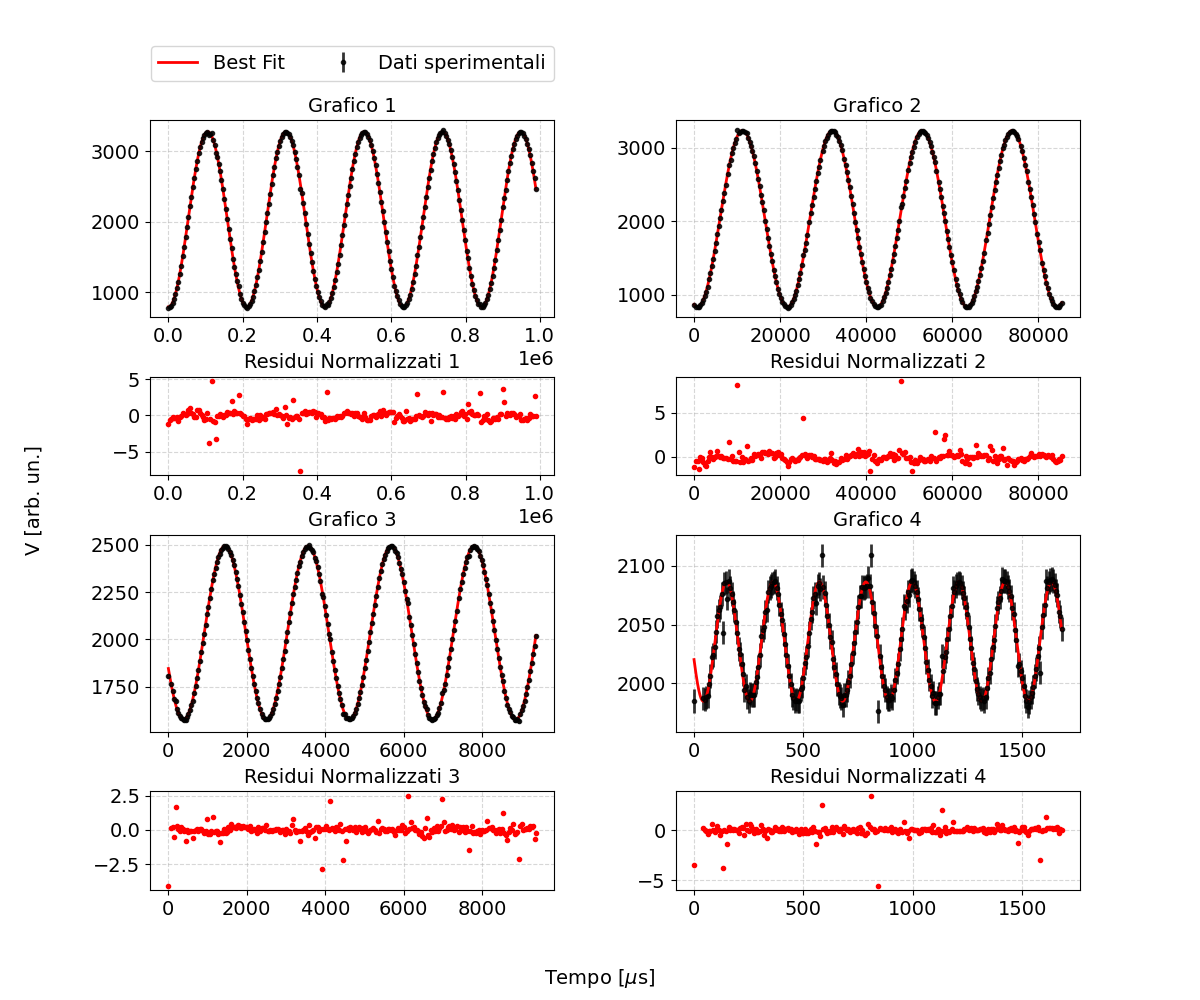
\includegraphics[width=0.85\textwidth]{bestfit_sinusoid.png} % Replace with your image name
                \caption{Grafici di bestfit nel caso di un'onda sinuosoidale che utilizza il modello descritto dall'Eq.(\ref{eq:fit_sin}).
                }
                \label{fig:bestfit_sinusoid}

            \end{figure}    



            \begin{table}[H]
                \centering
                \begin{tabular}{cccccc}
                    \hline
                               & Grafico1              &Grafico2               & Grafico3                &Grafico4 \\
                    \hline
                    $\omega$ [rad/s]    & $29.822\pm 0.003$     & $300.77 \pm 0.03$     & $2969.9\pm 0.7$         & $29652  \pm 3$ \\
                    $\delta$ [$\mu$s]   & $-1.588 \pm 0.001$    & $-1.811 \pm 0.001$    & $-2.723\pm 0.004$       & $-2.89 \pm 0.04$ \\
                    a [arb.un]          & $1240.2\pm 0.8$       & $1201.2\pm 0.9$        & $459.0 \pm 0.8$         & $50.8 \pm 0.8$ \\
                    c [arb.un]          & $2035.9 \pm 0.6$      & $2036.5 \pm 0.6$      & $2035.3 \pm 0.6$        & $2035.4 \pm 0.6$ \\
                    $\chi^{2}_{norm}$   & 0.009                 & 0.009                 & 0.002                   & 0.004 \\
                    \hline
                \end{tabular}
                \caption{Parametri ottenuti nei best-fit ottenuti nel caso di un'onda sinuosoidale. $\omega$ rappresenta la frequenza angolare, $\delta$ lo sfasamento, a l'ampiezza e c l'offset.}
                \label{tab:bestfit_sinusoid}
            \end{table}

    \subsection{Onda triangolare}
        \label{sez:bestfit_trian}
        E' stato realizzato il best-fit dei minimi quadrati
        di quattro set di dati compatibile con un'onda traingolare.
         Il modello con cui fare il best-fit è descritto dall'Eq.($\ref{eq:fit_trian}$).
            \begin{equation}
                x(t) = a\sum_{k=1,3,5...}^{1000} G(f,f_T)\frac{4}{(k\pi)^2}\sin\left(k\omega (t+\delta)+\phi(f,f_T)\right) +c
                \label{eq:fit_trian}
            \end{equation} 
        Dal $\chi^2$ risulta che l'errore è stato sovrastimato. 
        I parametri ottenuti sono riportati in Tab.(\ref{tab:bestfit_triangle}).%%%%%%%%%%%%%CHANGE TABLE
        In Fig.($\ref{fig:bestfit_triangle}$) sono graficati i dati con il best fit e 
        i residui. Dal $\chi^2$ possiamo dedurre che gli errori sono stati sovrastimati.
        Anche in questo caso,fatta eccezione del primo grafico,la frequenza di taglio aspettata 
        è compatibile entro una  barra di errore con quelle stimate.Il fatto che la prima stima  della
        frequenza  di taglio ,quella a frequenza più bassa,si discosti dalle altre suggerisce
        che il modello stia trascurando qualche fenomeno che a basse frequenze è incisivo.
        Siccome il circuito utilizzato per fare il campionamento dei dati era lo stesso, valgono le medesime considerazioni fatte in precedenza.
       
            \begin{figure}[H]            
                \centering
                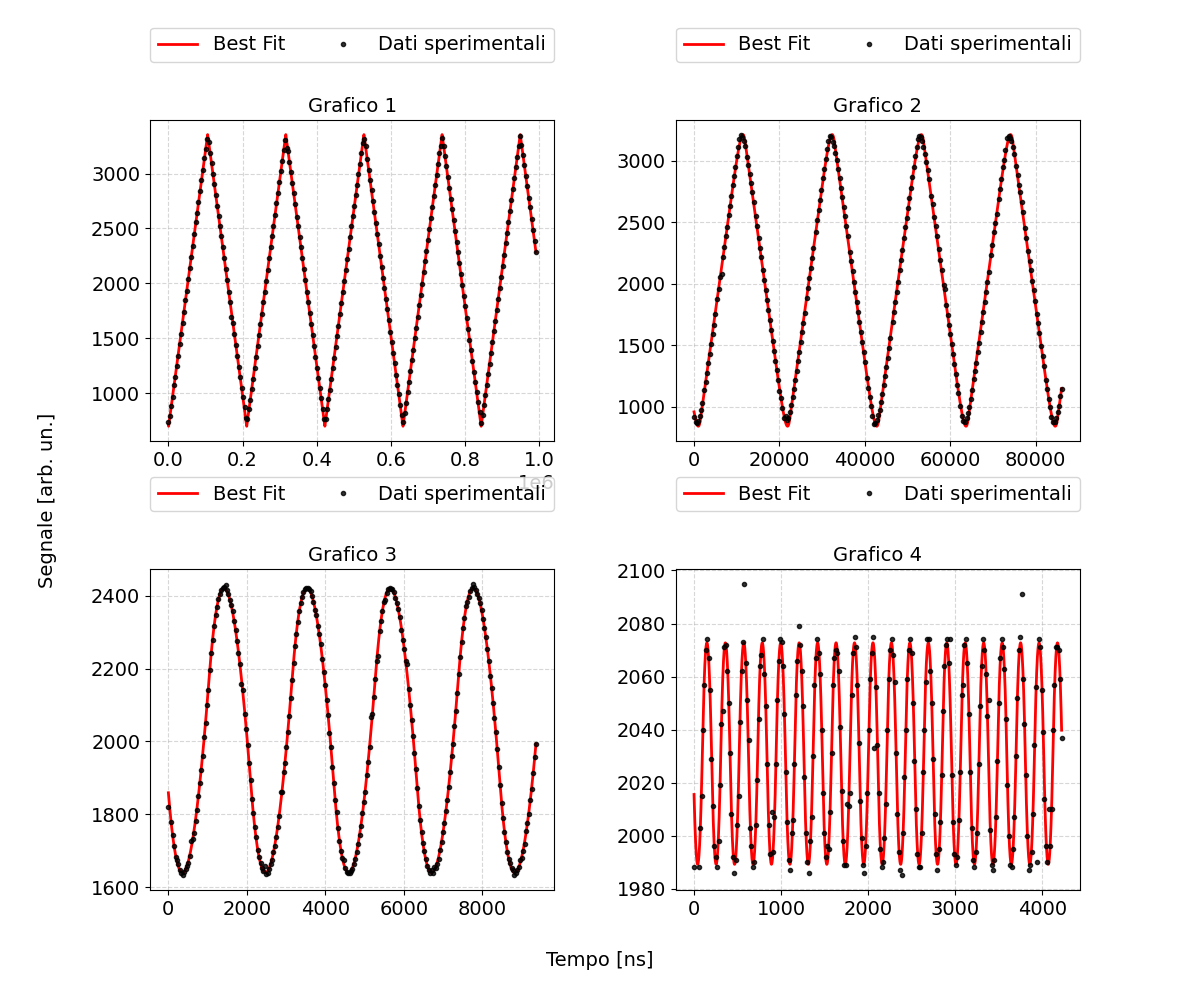
\includegraphics[width=0.85\textwidth]{bestfit_triangle.png} % Replace with your image name
                    \caption{Grafico di bestfit nel caso di un'onda triangolare che usa il modello descritto in Eq.(\ref{eq:fit_trian})
                }
                \label{fig:bestfit_triangle}
            \end{figure}    

            \begin{table}[H]
                \centering
                \begin{tabular}{cccccc}
                    \hline
                    Parametri           & Grafico1          &Grafico2               &Grafico3                   &Grafico4 \\
                    \hline
                    a [arb.un]          & $2665 \pm 3$      & $2671\pm 4$           & $2674\pm 139$             & $2652 \pm 12653$ \\
                    $\omega$ [rad/s]    & $29.817\pm 0.002$ & $300.784\pm 0.03$     & $2969.2\pm 0.08$          & $29667\pm 16$ \\
                    $\delta$ [s]        & $0.107\pm 0.002$  & $0.0105\pm 0.0001$    & $0.001073\pm 0.000007$    & $113\pm 7$ \\
                    c [arb.un]          & $2059.8 \pm 0.6$  & $1994.9 \pm 0.6$      & $2002.56 \pm 0.63$        & $2030.9 \pm 0.6$ \\
                    $f_T$ [$\mu$Hz]     & $61 \pm 4$        & $167 \pm 2$           & $187\pm 10$               & $189\pm 9$ \\
                    $\chi^{2}_{\text{norm}}$   & 0.007             & 0.006                 & 0.003                 & 0.0053 \\
                    \hline
                \end{tabular}
                \caption{Parametri ottenuti nei best-fit. $a$ è l'ampiezza del segnale, $\omega$ è la frequenza angolare del segnale, $\delta$ il duty cycle, $c$ l'offset dei nostri dati rispetto allo zero,
                $f_T$ la frequenza di taglio e $\chi^{2}_{\text{norm}}$ il chiquadro normalizzato.}
                \label{tab:bestfit_triangle}
            \end{table}

    \subsection{Treno di impulsi}
        E' stato realizzato il best-fit dei minimi quadrati
        di un set di dati compatibile con un treno di impulsi utilizzando il modello descritto in Eq.(\ref{eq:bestfit_train})
        \begin{equation}
            x(t) = a \left[\sum_{k=1}^{1000} \frac{2 G(f, f_T)}{k\pi} \sin{\left( k \pi \sigma \right)} \cos{\left((k \omega t) + \delta\right)}\right] + c
        \label{eq:bestfit_train}
        \end{equation}
        Riportiamo in Tab.(\ref{tab:bestfit_train}) i valori di bestfit ottenuti: in entrambi i casi c'è un $\chi^2$
        molto elevato dovuto alla presenza di punti sui transienti.
            \begin{figure}[H]            
                \centering
                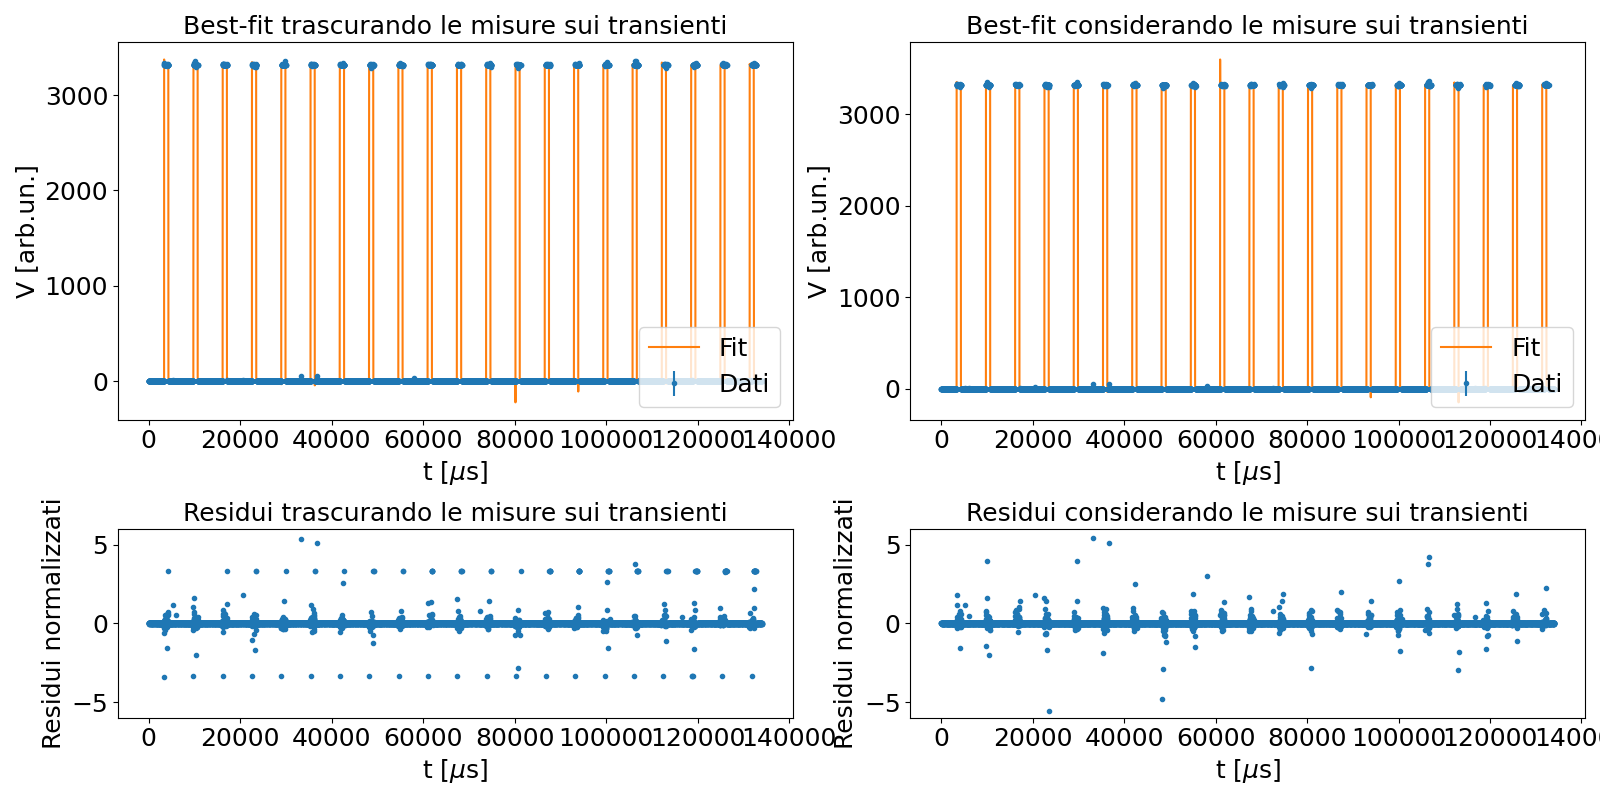
\includegraphics[width=1\textwidth]{bestfit_train.png} % Replace with your image name
                \caption{Grafico di bestfit nel caso di un treno di impulsi utilizzando il modello descritto in Eq.(\ref{eq:bestfit_train})
                }
                \label{fig:bestfit_train}
            \end{figure}    

            \begin{table}[H]
                \centering
                \begin{tabular}{ccc}
                    \hline
                               & Trascurando i transienti              &Considerando i transienti\\
                    \hline
                    a [arb.un]          & $3315 \pm 3$                          & $3312\pm 4$    \\
                    $\omega$ [rad/s]    & $981.7452\pm 0.0009$                  & $981.74\pm 0.04$ \\
                    $\delta$            & $0.145014\pm 0.000009$                & $0.14503\pm 0.00004$   \\
                    $\sigma$ [s]        & $-3870.016 \pm 0.002$                 & $-3869.9 \pm 0.3$  \\
                    $\chi^{2}_{\text{norm}}$   & 49                                    & 65 \\
                    \hline
                \end{tabular}
                \caption{Parametri ottenuti nei best-fit. $a$ rappresenta l'offset delle nostre misure rispetto allo zero, $\omega$ la frequenza angolare, $\delta$ il dutycycle ,$\sigma$ lo sfasamento e $\chi^2_{\text{norm}}$ è il chiquadro normalizzato}
                \label{tab:bestfit_train}
            \end{table}
\section{Simulazione numerica dei grafici guadagno vs frequenza}
    Sono stati eseguiti due bestfit per il guadagno del segnale periodico in uscita
     in funzione della frequenza in entrata, si vedano 
     Fig.($\ref{fig:image1}$) e Fig.($\ref{fig:image2}$). 
      I modelli utilizzati per effettuare i bestfit sono descritti da Eq.($\ref{eq:gain_square}$) 
      e da Eq.($\ref{eq:gain_trian}$) rispettivamente per l'onda quadrata e la triangolare. 
      Nel primo best fit è stato usato \emph{absolute\_ sigma=False} in quanto  
      sono stati usati dati acquisiti con l'oscilloscopio, soggetto ad errori sistematici.
      Nel secondo caso è stato usato \emph{absolute\_ sigma=True} in quanto i dati sono 
      stati estrapolati dal bestfit dell'onda triangolare fatto a in 
      Sez.($\ref{sez:bestfit_trian}$).
    
      \begin{equation}
        F(t, f) = a \left[\sum_{k=1}^n \frac{2}{k\pi} \frac{1}{\sqrt{1 + \left( \frac{f}{f_T} \right)^2}} \sin{\left(k\omega t + \arctan{\left(-\frac{f}{f_T}\right)} \right)}\right]
        \label{eq:gain_square}
    \end{equation}

    \begin{equation}
        F(t, f) = a \left[\sum_{k=1}^n \left( \frac{2}{k\pi} \right)^2 \frac{1}{\sqrt{1 + \left( \frac{f}{f_T} \right)^2}} \cos{\left( k\omega t + \arctan{\left(-\frac{f}{f_T}\right)} \right)}\right]
        \label{eq:gain_trian}
    \end{equation}
    
    $a$ e $f_T$ sono i parametri da stimati col bestfit. $a$ è un parametro di controllo che ci 
    aspettiamo essere 1. Tuttavia dai best fit Tab.($\ref{tab:results}$) questa richiesta non è attesa\\
    Come atteso, osserviamo che il guadagno di un'onda quadra è maggiore rispetto a quello di un'onda triangolare. 
        \begin{figure}[htbp]
            \centering
            \begin{subfigure}{0.45\textwidth} % Adjust width as needed
                \centering
                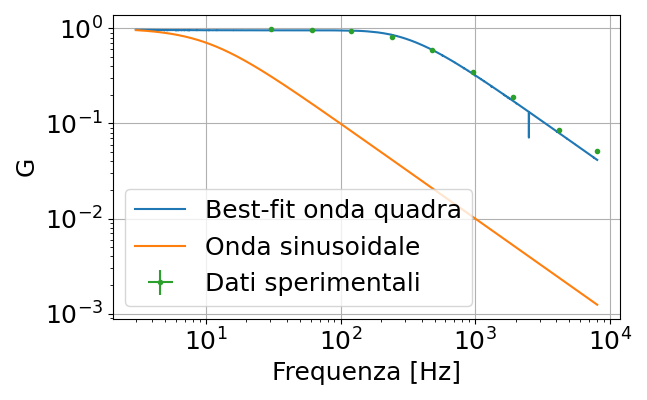
\includegraphics[width=\textwidth]{gain_squarewave.png} % Replace with your image path
                \caption{}
                \label{fig:image1}
            \end{subfigure}
            \hfill % Adds spacing between images
            \begin{subfigure}{0.45\textwidth} % Adjust width as needed
                \centering
                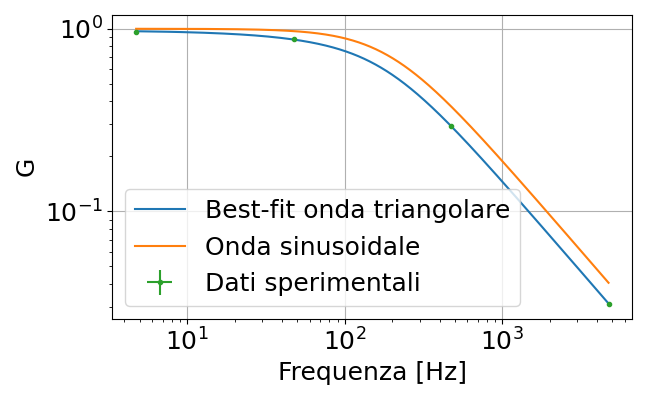
\includegraphics[width=\textwidth]{gain_trianwave.png} % Replace with your image path
                \caption{}
                \label{fig:image2}
            \end{subfigure}
            \caption{(a),(b): Bestfit del guadagno in funzione della frequenza in ingresso nel caso di un'onda quadra e di un'onda triangolare}
            \label{fig:side_by_side_images}
        \end{figure}

        \noindent Riportiamo i valori di bestfit in Tab.(\ref{tab:results}).La frequenza di taglio, per l'onda triangolare è
        in accordo con quanto aspettato, ma non con i best fit realizzati in Sez.($\ref{sez:bestfit_trian}$) .
        Nel caso dell'onda quadra non c'è accordo con la misura effettuata in laboratorio della frequenza di taglio: $f_{t}=(340.4\pm0.1)$ $\mu$Hz. 

        \begin{table}[H]
            \centering
            \begin{tabular}{ccc}
                \hline
                            &Onda quadra        & Onda triangolare\\
                \hline
                $f_T$[$\mu$Hz]  &$191.6\pm0.9$      & $222\pm1$\\
                $a$         &$0.979\pm0.002$    &   $0.951\pm0.002$\\
                $\kappa^2$        & $52   $             &   $1$ \\
            
                \hline
            \end{tabular}
            \caption{Parametri stimati dal bestfit del guadagno in funzione della frequenza in ingresso. $f_T$ è la frequenza di taglio, }
            \label{tab:results}
        \end{table}
        \bibliographystyle{plain}
        \bibliography{main.bib}
\end{document}